\subsection{Level Set}

The main purpose of this report is to liquid fluids and especially water. Liquid fluids, unlikey gas fluids, have a surface. Tracking a surface is a non-trivial problem to solve due to the complex shape and the evolving change of topology. It is important to get the surface tracking as good as possible. Later on we need to know if a grid cell is inside, outside or on the surcface when solving for pressure. To track the surface, we will use a level set. A level set is a grid approach to track a surface. At each cell in the grid, a scalar $\phi_{i,j}$ is stored. This absolute value of the scalar tells us the closest distance to the surface. To know if we are inside, outside or on the actual surface we use the following notation

\begin{equation}
\phi = 
\left\{
\begin{array}{ll}
\phi < 0 & \mbox{inside}  \\
\phi > 0 & \mbox{outside} \\
\phi = 0 & \mbox{surface} \\
\end{array}
\right.
\end{equation}

Figure \ref{levetsetexample} shows an example of a surface and an interior and exterior area. Notice that if the surface is right on the center of a cell, then $\phi$ is zero. 

\begin{figure}[ht!]
\centering
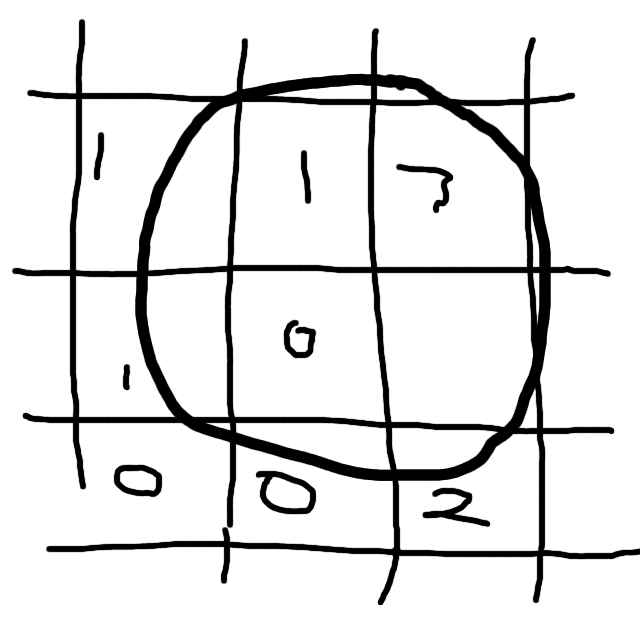
\includegraphics[width=90mm]{ch2/levelset.png}
\caption{A simple caption}
\label{levetsetexample}
\end{figure}

Another important feature of a level set is the gradient.

\begin{equation}
\nabla \phi = \hat{n}
\end{equation}

where $\hat{n}$ is the direction to the closest point of the surface. This means, given patial coordinates $\vec{x}$, one can easily find the closest point $\vec{x}_s$ on the surface. 

\begin{equation}
\vec{x}_s = \vec{x} - \phi(\vec{x})\nabla \phi(\vec{x})
\end{equation}

For this math to work, it is important that the following condition is always met:

\begin{equation}
|\phi| = 1
\end{equation}

This is called the Eikonal equation and is fundamental for any of the level set operations. 
